\section*{Path and trajectory planning}
\subsection*{Difference between path and trajectory}
(Something about the difference)\\


Now that the problem of inverse kinematics is solved and a functioning controller is made, it is time for to generate a motion. The first thing that is easiest to do is to create a 1D motion of the robot. In this test case the robot is to move up and down in the z direction. Therefore a sine function is created and then sent to the inverse kinematic solver to generate the joint angles for each position. The solution for one position is used as the initial point for the next position to avoid too much time consumption and try to avoid that it finds another solution to the problem. In \figref{fig:joint2Sin} the calculated joint angles is shown. Unfortunately one can see that the solver changes between two solution paths. In this case one can see that the solver favors one path over the other which means in this case it should be easy to fill in the missing parts of the motion. In other cases it may be very difficult or impossible to do this. Another problem is to determine what path are corresponding to the same motion and how to distinguish between them. 
%(NOTE: calculating this path with 63 points takes 268 seconds. Matlab uses only one core calculating this. Matlab has a parfor loop which uses parallell computing and all 4 cores. For obvious reason one cannot use the previous solution as the initial point and the results are very bad. It uses 90 seconds)

\begin{figure}[htbp]
  \centering
  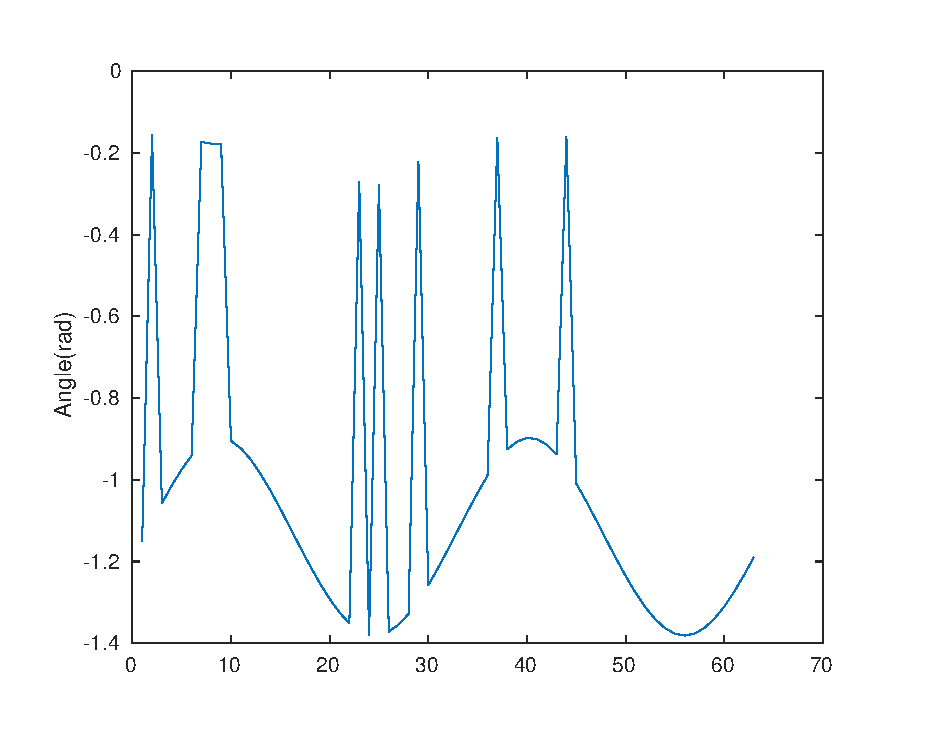
\includegraphics[width=.9\textwidth]{img/joint2SinMove.eps}
  \caption{The calculated joint angles for the second joint when a sine movement in the z direction(world frame) is wanted}
  \label{fig:joint2Sin}
\end{figure}

Because of the simplicity of the movement it is easy to manually curvefit the right part of the desired joint angles. In \figref{fig:manCur} the curvefitted function is seen. It is not perfect it works well enough to test the solution for this case. Further work on this will include a process to automatically fix this problem. 


\begin{figure}[htbp]
  \centering
  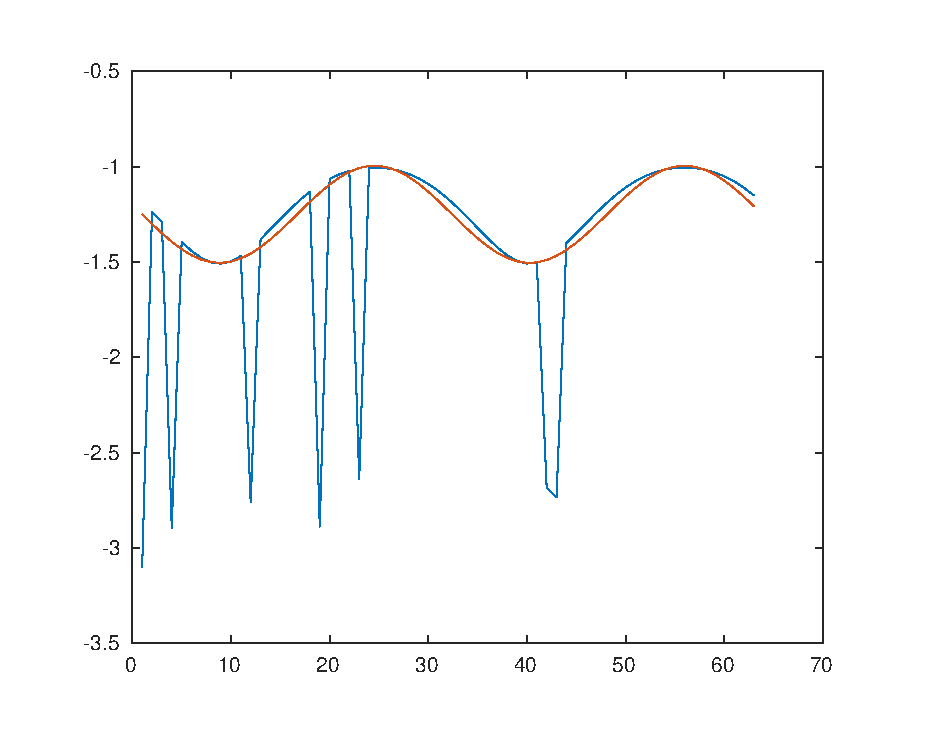
\includegraphics[width=.9\textwidth]{img/manCurvfit.eps}
  \caption{Manually curve fitted joint position}
  \label{fig:manCur}
\end{figure}



\begin{figure}[htbp]
  \centering
  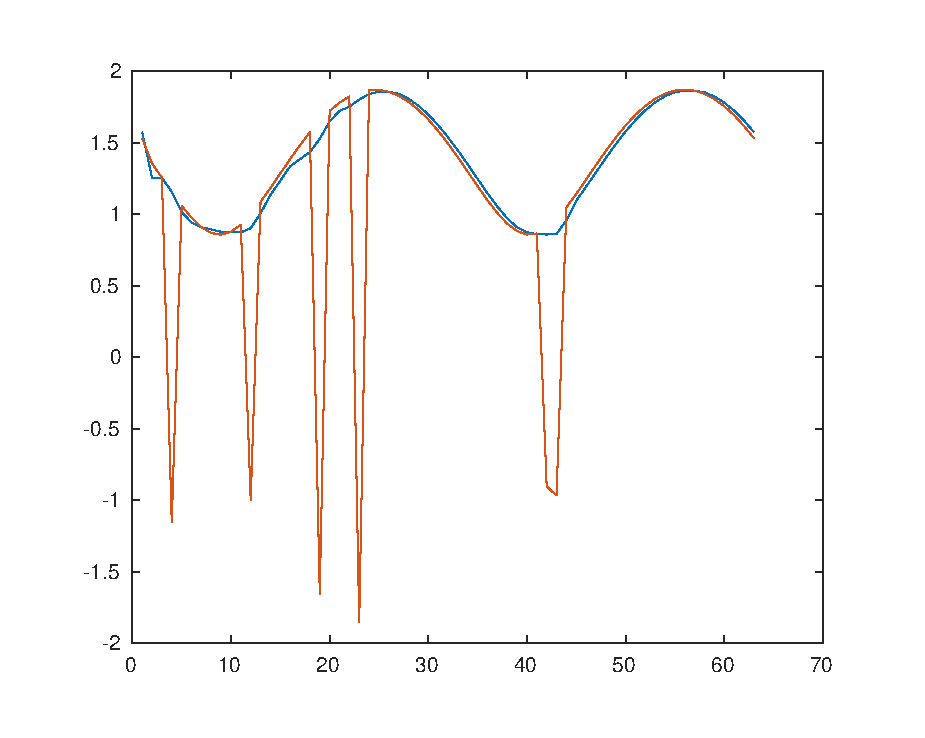
\includegraphics[width=.9\textwidth]{img/medAvgFilt.eps}
  \caption{Median and average filtered angle}
  \label{fig:manCur}
\end{figure}